% one-figure manuscript written by fig_qc.py --tek-sekil-tex (trap T29)
\begin{figure}[!t]
\centering
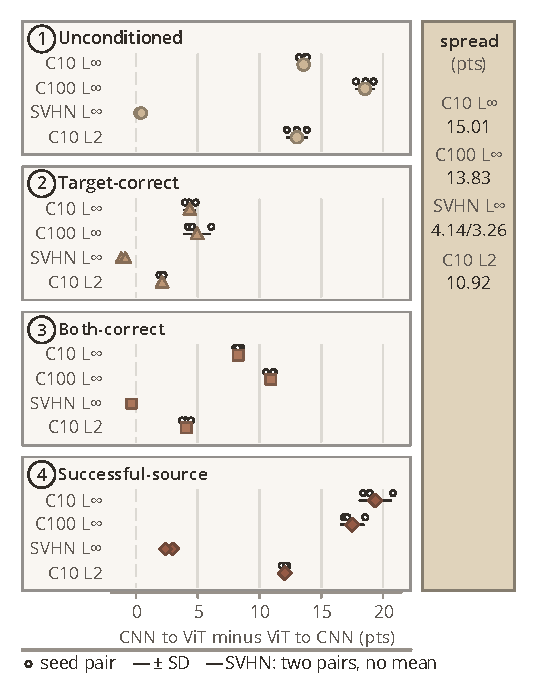
\includegraphics{fig13_protocol_settings}
\caption{\textbf{Protocol by setting as four exploded boards.} Transfer asymmetry (CNN to ViT minus ViT to CNN): boards 1-4 are the conditioning protocols, set back layer by layer; rows are settings, mean±SD over three seed pairs, pairs as small circles (SVHN two, no mean). Values are positions on each board's flat face; the spine prints the spread.}
\label{fig:fig13_protocol_settings}
\end{figure}
